\documentclass[UTF8]{beamer}
% \usepackage{ctex}
\usepackage{graphicx}
\usepackage{amsmath}
\usepackage{bookmark}
\usepackage{color}
\usepackage{animate}
\usepackage{animate}
\usepackage{subfigure}
\usepackage{enumerate}
\usepackage{geometry}
\usepackage{float}
\usepackage{cite}
\usepackage{listings}

\usetheme{cambridgeUS}
\usefonttheme[onlymath]{serif}

\author{Zerui Liu}
\institute{NAOC}
\title{Fisher Matrix Forecast of HI IM FAST}

\date{\today}

\begin{document}
\begin{frame}
    \maketitle
    
\end{frame}
\begin{frame}
    \frametitle{Detectbility and Fisher Matrix Forecast}

    The total brightness temperature is given by
    \begin{equation}
        \delta T(\vec{\theta}_p,\nu_p) = \delta T^S(\vec{\theta}_p,\nu_p)+\delta T^N(\vec{\theta}_p,\nu_p)+\delta T^F(\vec{\theta}_p,\nu_p)
    \end{equation}
    Fourier Transfomation
    \begin{equation}
        <\delta T^{X*}(\vec{q},y)\delta T^{X'}(\vec{q}',y')> = (2\pi^3)C^X(\vec{q},y)\delta^2(\vec{q}-\vec{q}')\delta(y-y')\delta_{XX'}
    \end{equation}
    For signal:
    \begin{equation} 
        T_b = \bar{T}_b(1+\delta_{HI})
    \end{equation}
    \begin{equation}
        \bar{T_b} = \frac{3}{32}\frac{hc^3A_{10}}{k_Bm_p\nu_{21cm}}\frac{(1+z)^2}{H(z)}\Omega_{HI}(z)\rho_{c,0}
    \end{equation}       
\end{frame}
\begin{frame}     
    
    \begin{equation}
        \delta_{HI}(\vec{k})=(b_{HI}+f\nu^2)\exp(-k^2\mu^2\sigma_{NL}^2/2)\delta_M(\vec{k})
    \end{equation}
    And
    \begin{equation}
       <\delta_M^* \delta_M>=(2\pi)^3 P(\vec{k})\delta^3(\vec{k}-\vec{k}')
    \end{equation}     
    So signal covariance is 
    \begin{equation}
        C^S(\vec{q},y)=T_b^2(z_i)\frac{P_{tot}}{r^2r_\nu}
    \end{equation}
    \begin{equation}
        P_{tot}=F_{RSD}(\vec{k}_{\perp},k_{\parallel})D_{z}^2P(k,z=0)
    \end{equation}
    \begin{equation}
        F_{RSD}=(b_{HI}+f\mu^2)^2\exp (-k^2\mu^2\sigma_{NL}^2)
    \end{equation}
\end{frame}
\begin{frame}
    \frametitle{Noise model}
    \begin{equation}
        C^{N}(q,y)=\frac{T_{sys}^2}{t_{tot}\Delta \nu}U_{bin}\mathcal{L}B_{\perp}^{-2}B_{\parallel}^{-1}
    \end{equation}
    $T_{sys}$: system temperature; $t_{tot}$: total integration time; $U_{bin}=S_{area\Delta\tilde{nu}}$: the volume of an individual redshift bin; $S_{area}$: survey area; $
    Delta \tilde{\nu}$: (dimensionless) bandwidth
    \begin{equation}
        B_{\parallel}=\exp(-\frac{(y\delta\nu/\nu_{21cm})^2}{16\ln 2})
    \end{equation}
    For single dish
    \begin{equation}
        \mathcal{L}=\frac{f(\nu)}{N_bN_d}
    \end{equation}
    \begin{equation}
        B_{\perp}=\exp(-\frac{(q\theta_B)^2}{16\ln 2})
    \end{equation}
    
\end{frame}
\begin{frame}
    For interferometers
    \begin{equation}
        \mathcal{L}B_{\perp}^{-2}=\frac{FOV}{n(u=q/2\pi)}
    \end{equation}
    \begin{equation}
        n(u)=\frac{N_d(N_d-1)}{2\pi(u_{max}^2-u_{min}^2)}
    \end{equation}
\end{frame}
\begin{frame}
    \frametitle{Foreground model}
    \begin{equation}
        C^F(\vec{q},y)=\epsilon^2\sum_{X}A_{X}(\frac{l_p}{2\pi q})^{nx}(\frac{\nu_p}{\nu_i})^{mx}
    \end{equation}
    \begin{table}[]
        \begin{tabular}{l|lll}
        \hline
        Foreground                  & $A_X/mK^2$ & $n_x$                    & $m_x$                     \\ \hline
        Extragalactic point sources & 57.0       & 1.1                      & 2.07                      \\
        Extragalactic free-free     & 0.014      & 1.0                      & 2.10                      \\
        Galactic synchrotron        & 700        & 2.4                      & 2.80                      \\ 
        Galactic free-free          & 0.088      & 3.0 & 2.15 \\ \hline
        \end{tabular}
    \end{table}
\end{frame}
\begin{frame}
    \frametitle{Fisher Matrix Forecast}
    \begin{equation}
        F_{ij}^{IM} = \frac{1}{2}U_{bin}\int\frac{d^2qdy}{(2\pi)^3}[\partial_i \ln C^T(\vec{q},y)\partial_j \ln C^{T}(\vec{q},y)]
    \end{equation}
    For the uncertainty of power spectrum
    \begin{equation}
        (\frac{\Delta P_a}{P_a})^2=[\frac{1}{2}U_{bin}\int_{V_n}\frac{d^2qdy}{(2\pi^3)}(\frac{C^S(\vec{q},y)}{C^T(\vec{q},y)})^2]^{-1}
    \end{equation}
    Pipeline of Fisher Forecast: Philip Bull, Pedro G. Ferreira, Prina Patel, and Mario Santos, ApJ 803, 21 (2015) [arXiv:1405.1452][doi:10.1088/0004-637X/803/1/21].
\end{frame}
    \begin{frame}
        \frametitle{Cosmology model}
        scale factor $a = \frac{1}{1+z}$,and Hubble Constant $H(t)=\frac{\dot{a}}{a}$
        \begin{equation}
            H^2 = \frac{8\pi G}{3}\rho -\frac{kc^2}{a^2}+\frac{\Lambda c^2}{3}
        \end{equation}
        \begin{equation}
            H(a)=\frac{\dot{a}}{a}=H_0\sqrt{(\Omega_c+\Omega_b)a^{-3}+\Omega_{rad}a^{-4}+\Omega_k a^{-2}+\Omega a^{-3(1+\omega)}}
        \end{equation}
        \begin{equation}
            H^2(a)=H_0^2[\omega_R a^{-4}+\Omega_M a^{-3}+\Omega_ka^{-2}+\Omega_{DE}\exp \{3\int_a^1\frac{da'}{a'}[1+\omega(a')] \}]
        \end{equation}
        Cosmological Constant
        \begin{equation}
            \{ h,\Omega_b h^2, \omega_DE, \Omega_K,\omega_0, \omega_a, n_s,\sigma_8 \}
        \end{equation}
    \end{frame}
    \begin{frame}
        Cosmological Constant
        \begin{equation}
            \{ h,\Omega_b h^2, \omega_DE, \Omega_K,\omega_0, \omega_a, n_s,\sigma_8 \}
        \end{equation}
        \begin{itemize}
            \item $n_s$ is the spectral index of the scalar power spectrum($P(k)\sim k^{n_s-1}$). $\sigma_8$ is the amplitude of the power spectrum on the scale of 8 Mpc/h.
            \item $\omega_a = \omega_0+(1-a)\omega_a$
        \end{itemize}
        
        
    \end{frame}
    \begin{frame}
        \frametitle{HI intensity mapping survey}
        \begin{table}[]
            \begin{tabular}{l|llll}
            \hline
                                               & FAST   & MeerKATb1 & MeerKATb2 & FASTWB \\ \hline
            Total integration time/h             & 100000 & 4000          & 4000          &    -           \\
            Ndish                              & 1      & 64            & 64            & 1              \\
            Nbeam                              & 19     & 1             & 1             & 1              \\
            Ddish/m                              & 300    & 13.5          & 13.5          & 300            \\
            System Temp./mK                 & 20     & 29            & 20            & 60             \\
            Total bandwidth/MHz                    & 300    & 435           & 520           & -              \\
            Max frequency/MHz                      & 1350   & 1015          & 1420          & 1050           \\
            Survey area/$deg^2$ & 20000  & 4000          & 4000          &     -          \\ \hline
            \end{tabular}
            \end{table}
    \end{frame}
    \begin{frame}
        \frametitle{resolution}
        \begin{figure}
            \centering
            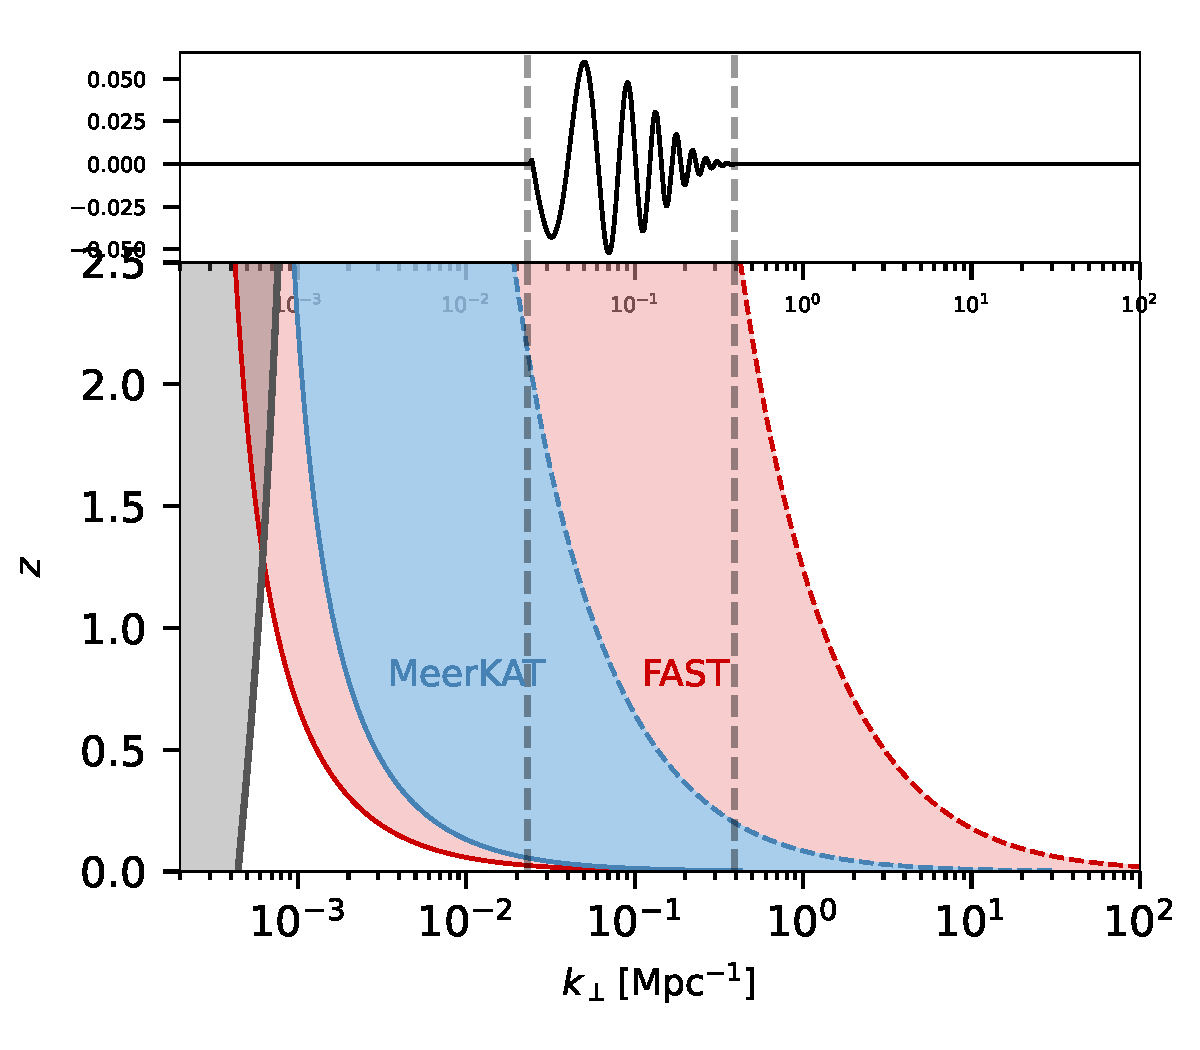
\includegraphics[scale=0.4]{fig03-resolution-z.pdf}
        \end{figure}
    \end{frame}
    
    \begin{frame}
        \frametitle{}
        \begin{figure}
            \centering
            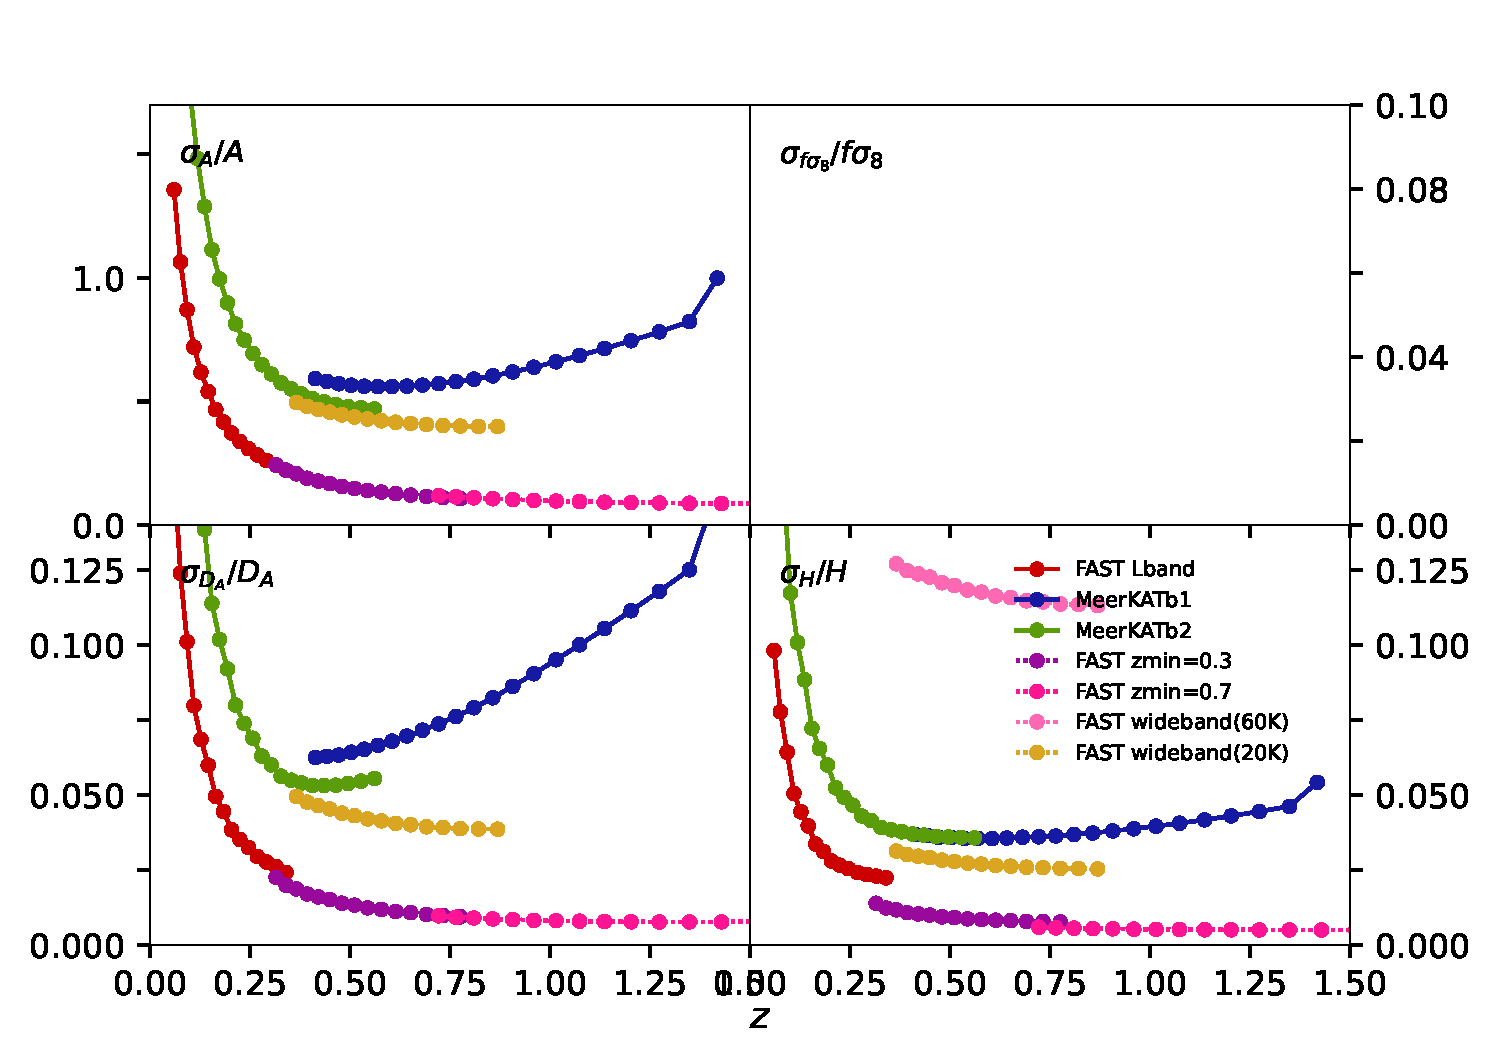
\includegraphics[scale=0.4]{fig06-zfns.pdf}
            \caption{Fractional errors on $A(z)$, $f\sigma_8(z)$(with a bug), $D_A(z)$, and $H(z)$, as a function of redshift}
        \end{figure}
    \end{frame}

    \begin{frame}
        \frametitle{}
        \begin{figure}
            \centering
            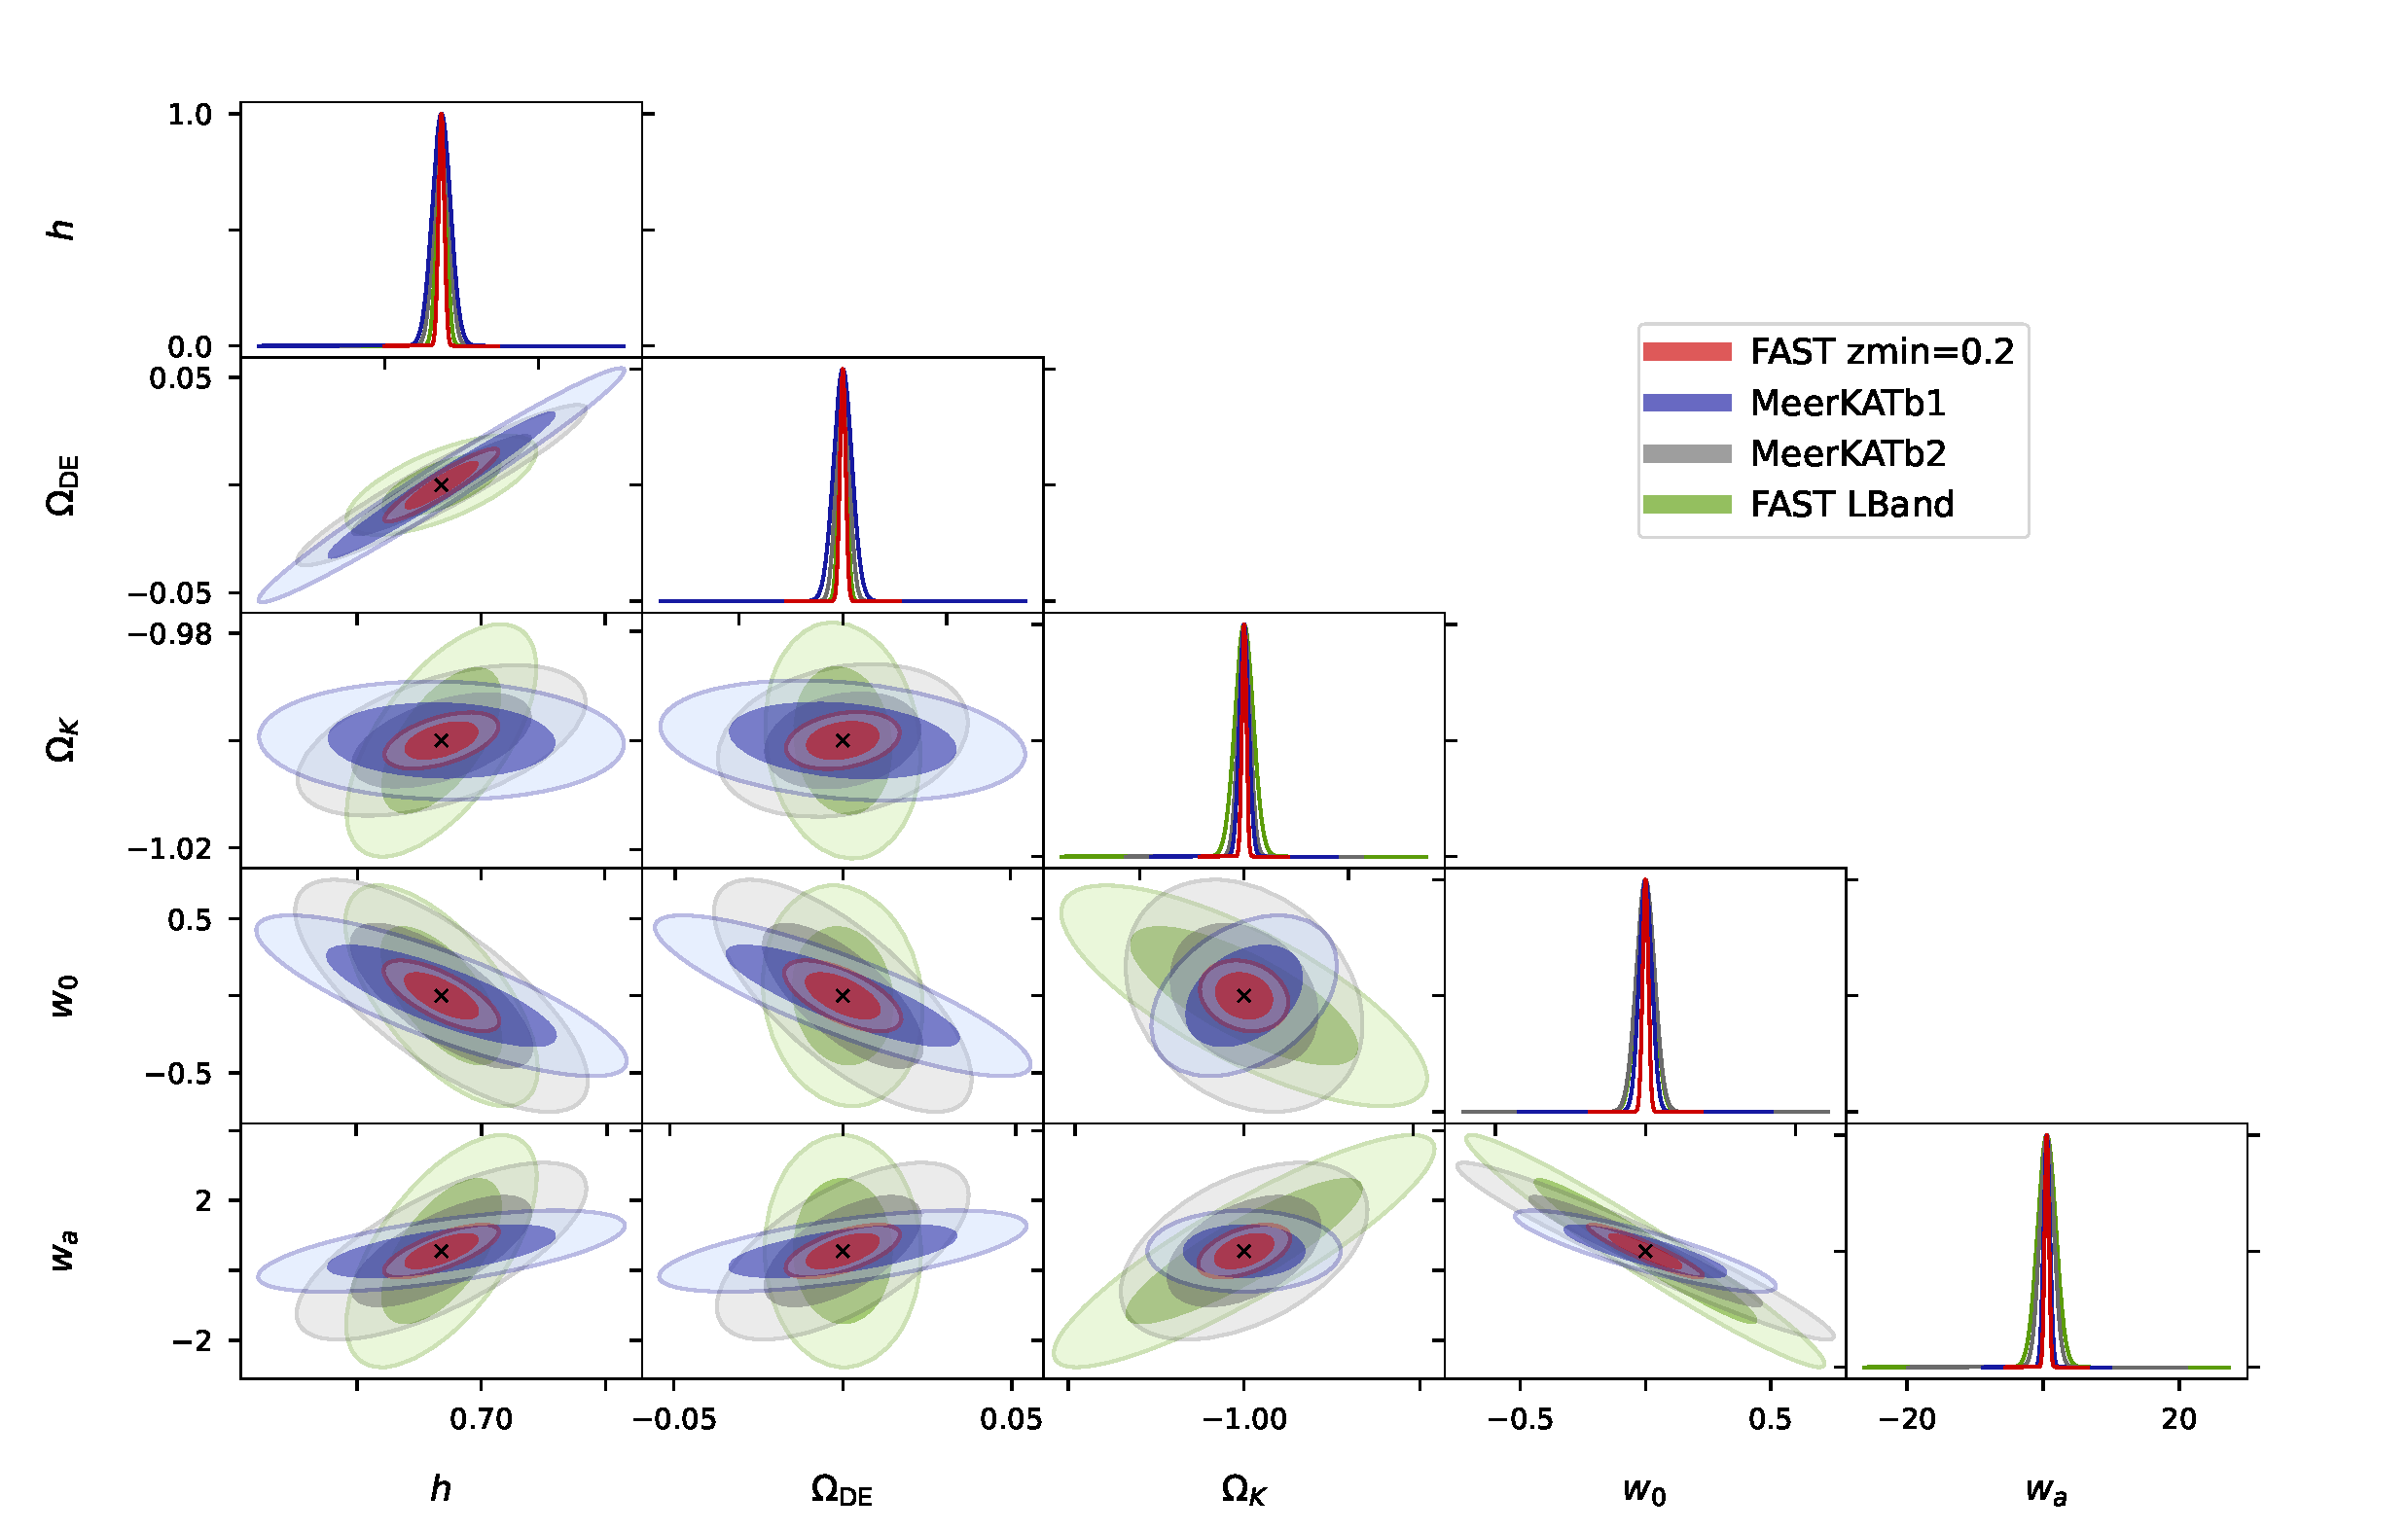
\includegraphics[scale=0.27]{fig17-6params-eos.pdf}
            \caption{Forecasts for dark energy and modified growth parameters (without $\gamma$)}
        \end{figure}
    \end{frame}

    \begin{frame}
        \frametitle{}
        \begin{columns}[c]
            \column{0.5\linewidth}
            \begin{figure}
                \centering
                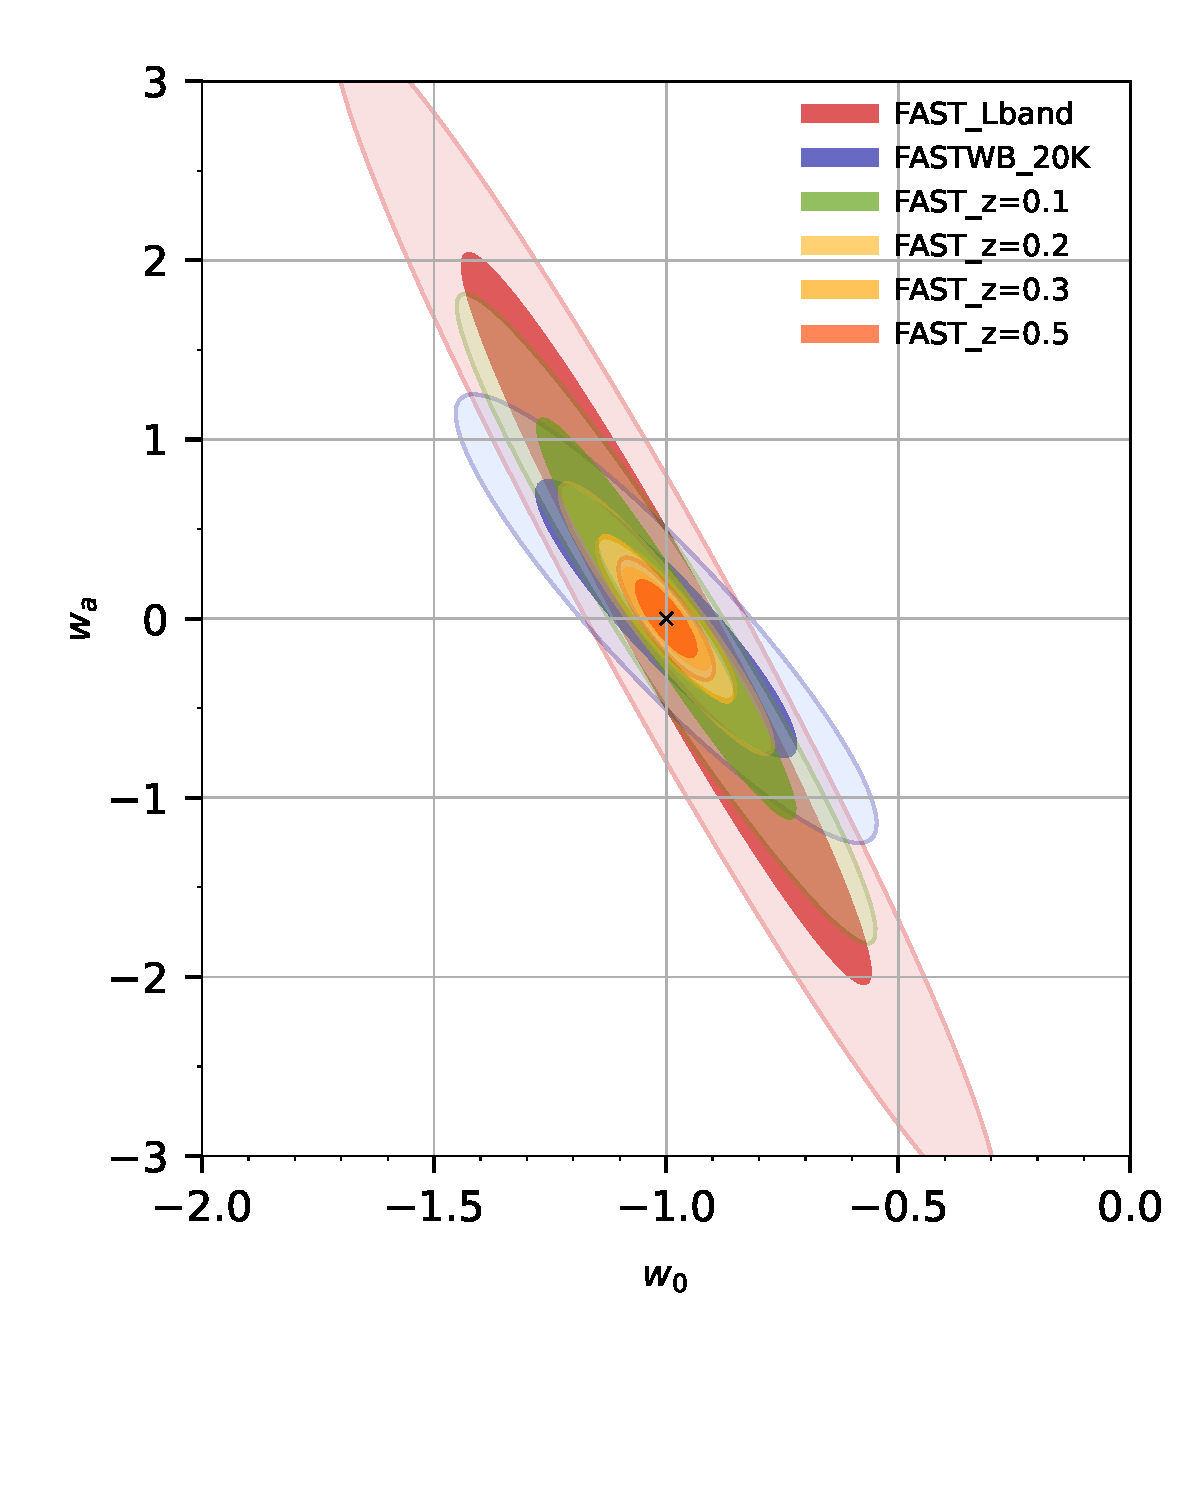
\includegraphics[scale=0.3]{test-w0wa-bandwidth300MHz.pdf}
            \end{figure}
            \column{0.5\linewidth}
            \begin{table}[]
                \begin{tabular}{l|ll}
                \hline
                                     & $\sigma_{\omega_0}$ & $\sigma_{\omega_a}$ \\ \hline
                FAST\_Lband          & 0.28                & 1.33                \\
                FAST zmin=0.1        & 0.182               & 0.7314              \\
                FAST zmin=0.2        & 0.0927              & 0.3047              \\
                FAST zmin=0.3        & 0.0603              & 0.1832              \\
                FAST zmin=0.5        & 0.0416              & 0.1376              \\
                FAST wb(20K) & 0.2365              & 0.6975              \\ \hline
                \end{tabular}
            \end{table}
            FAST: $t_{int}=48(1+z) s/pix$
            
            total bandwidth=300Hz

            $S_{area} = 20000deg^2$
        \end{columns}
    \end{frame}

    \begin{frame}
        \frametitle{}
        \begin{columns}[c]
            \column{0.5\linewidth}
            \begin{figure}
                \centering
                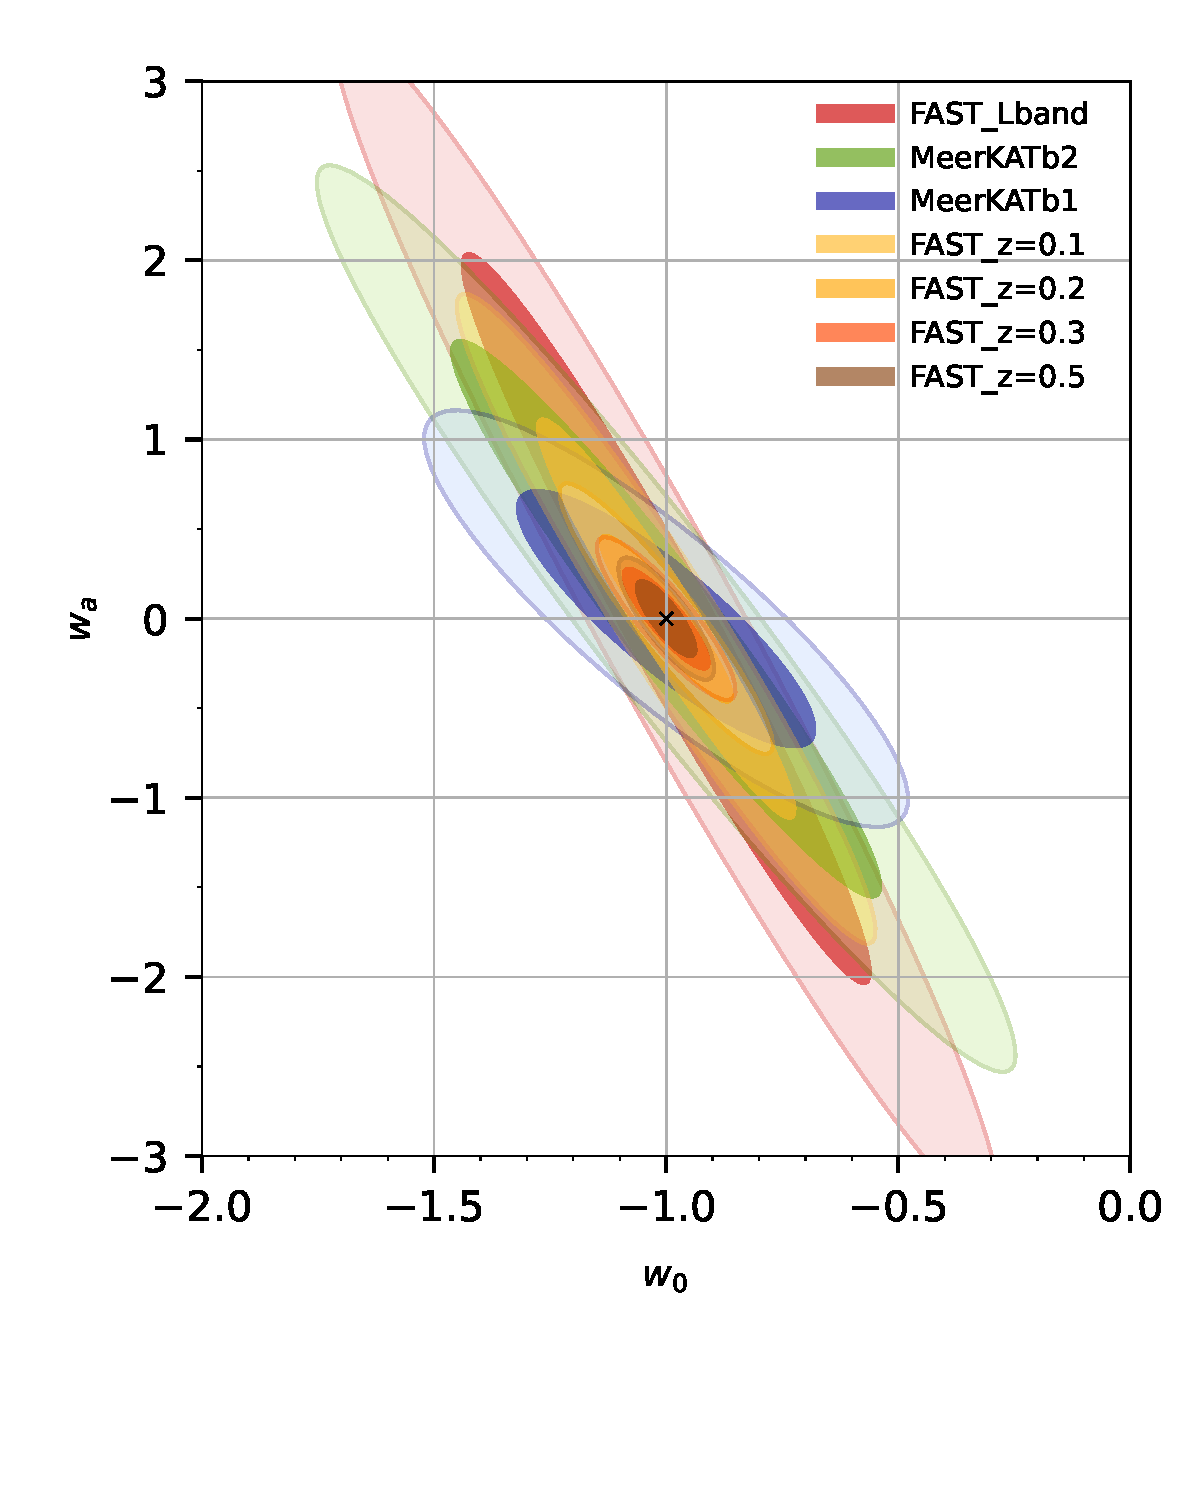
\includegraphics[scale=0.3]{test-w0wa-withMeerKAT.pdf}
            \end{figure}
            \column{0.5\linewidth}
            \begin{table}[]
                \begin{tabular}{l|ll}
                \hline
                                     & $\sigma_{\omega_0}$ & $\sigma_{\omega_a}$ \\ \hline
                FAST\_Lband          & 0.28                & 1.33                \\
                MeerKAT\_b1          & 0.2103              & 0.4689              \\
                MeerKAT\_b2          & 0.3036              & 1.0204              \\
                FAST zmin=0.1        & 0.182               & 0.7314              \\
                FAST zmin=0.2        & 0.0927              & 0.3047              \\
                FAST zmin=0.3        & 0.0603              & 0.1832              \\
                FAST zmin=0.5        & 0.0416              & 0.1376              \\ \hline
                \end{tabular}
                \end{table}
        \end{columns}
    \end{frame}
    \begin{frame}
        \frametitle{}
        \begin{columns}[c]
            \column{0.5\linewidth}
            \begin{figure}
                \centering
                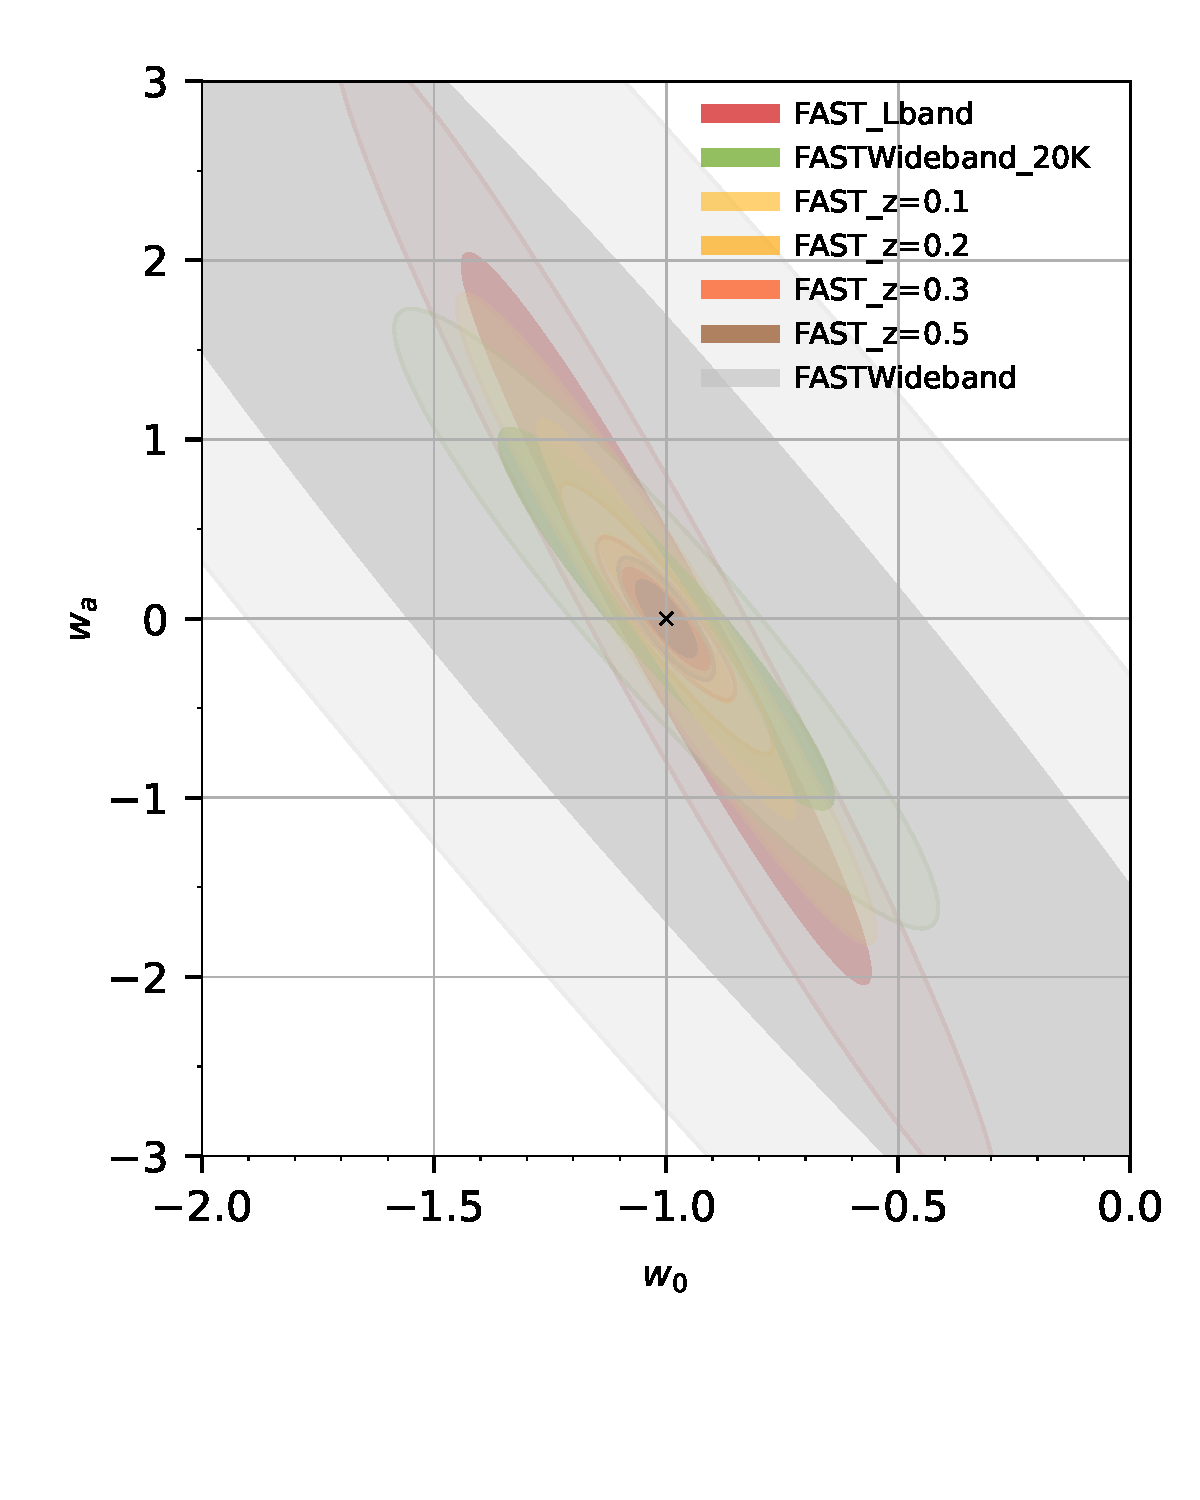
\includegraphics[scale=0.3]{test-w0wa_withwideband.pdf}
            \end{figure}
            \column{0.5\linewidth}
            \begin{table}[]
                \begin{tabular}{l|ll}
                \hline
                                     & $\sigma_{\omega_0}$ & $\sigma_{\omega_a}$ \\ \hline
                FAST\_Lband          & 0.28                & 1.33                \\
                FAST zmin=0.1        & 0.182               & 0.7314              \\
                FAST zmin=0.2        & 0.0927              & 0.3047              \\
                FAST zmin=0.3        & 0.0603              & 0.1832              \\
                FAST zmin=0.5        & 0.0416              & 0.1376              \\
                FAST wb(60K)        & 1.1732              & 3.5682              \\
                FAST wb(20K) & 0.2365              & 0.6975              \\ \hline
                \end{tabular}
                \end{table}
        \end{columns}
    \end{frame}

    \begin{frame}
        \frametitle{NEXT}
        \begin{itemize}
            \item increase integration time
            \item decrease $S_{area}$
        \end{itemize}
    \end{frame}

    \begin{frame}
        \frametitle{Resolution, add Tianlai}
        \begin{figure}
            \centering
            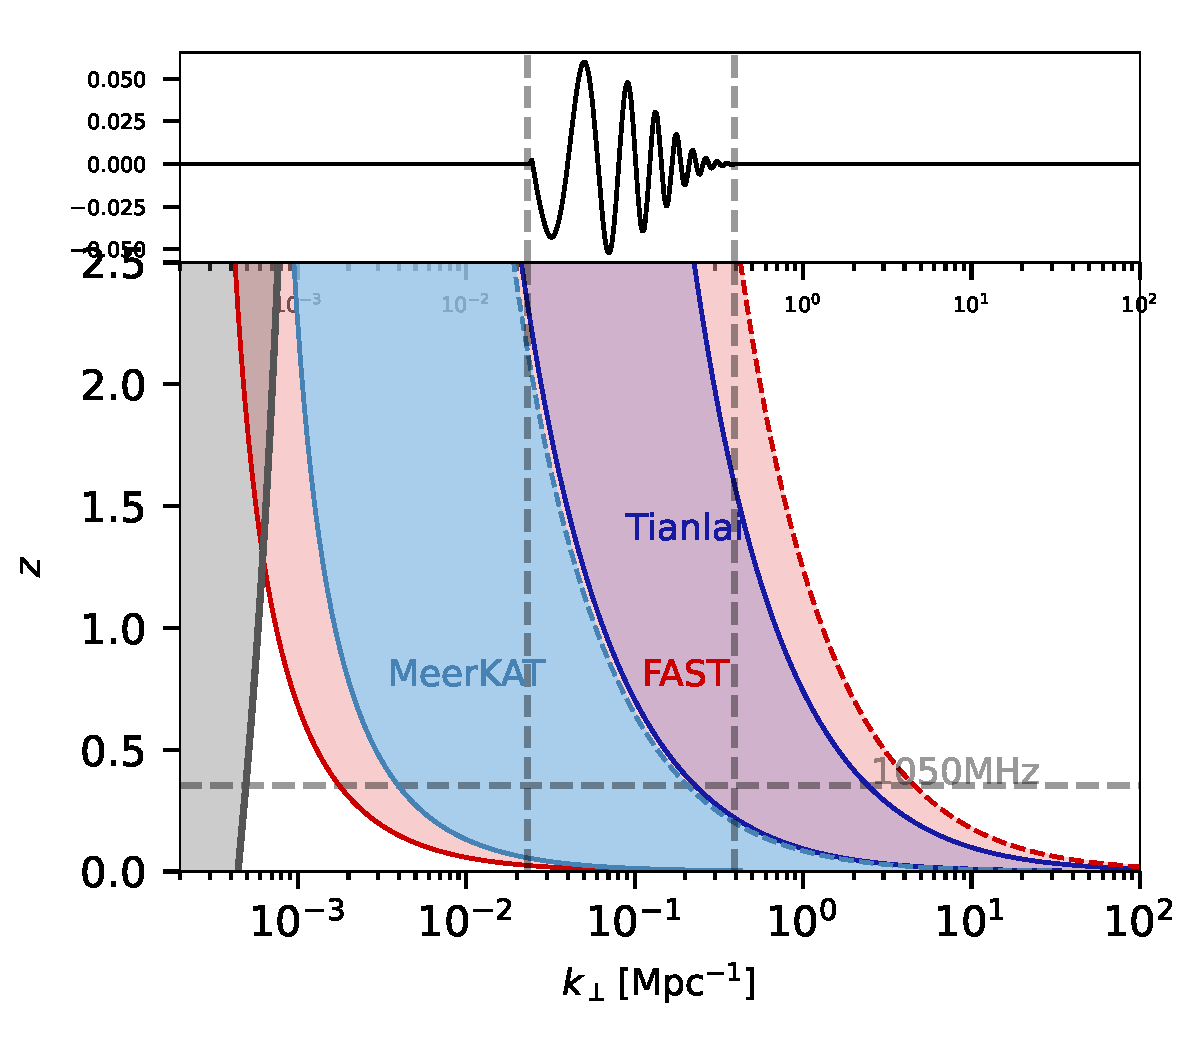
\includegraphics[scale=0.4]{fig03-resolution-z-withTianlai.pdf}
        \end{figure}
    \end{frame}
    
    \begin{frame}
        \frametitle{}
        \begin{figure}
            \centering
            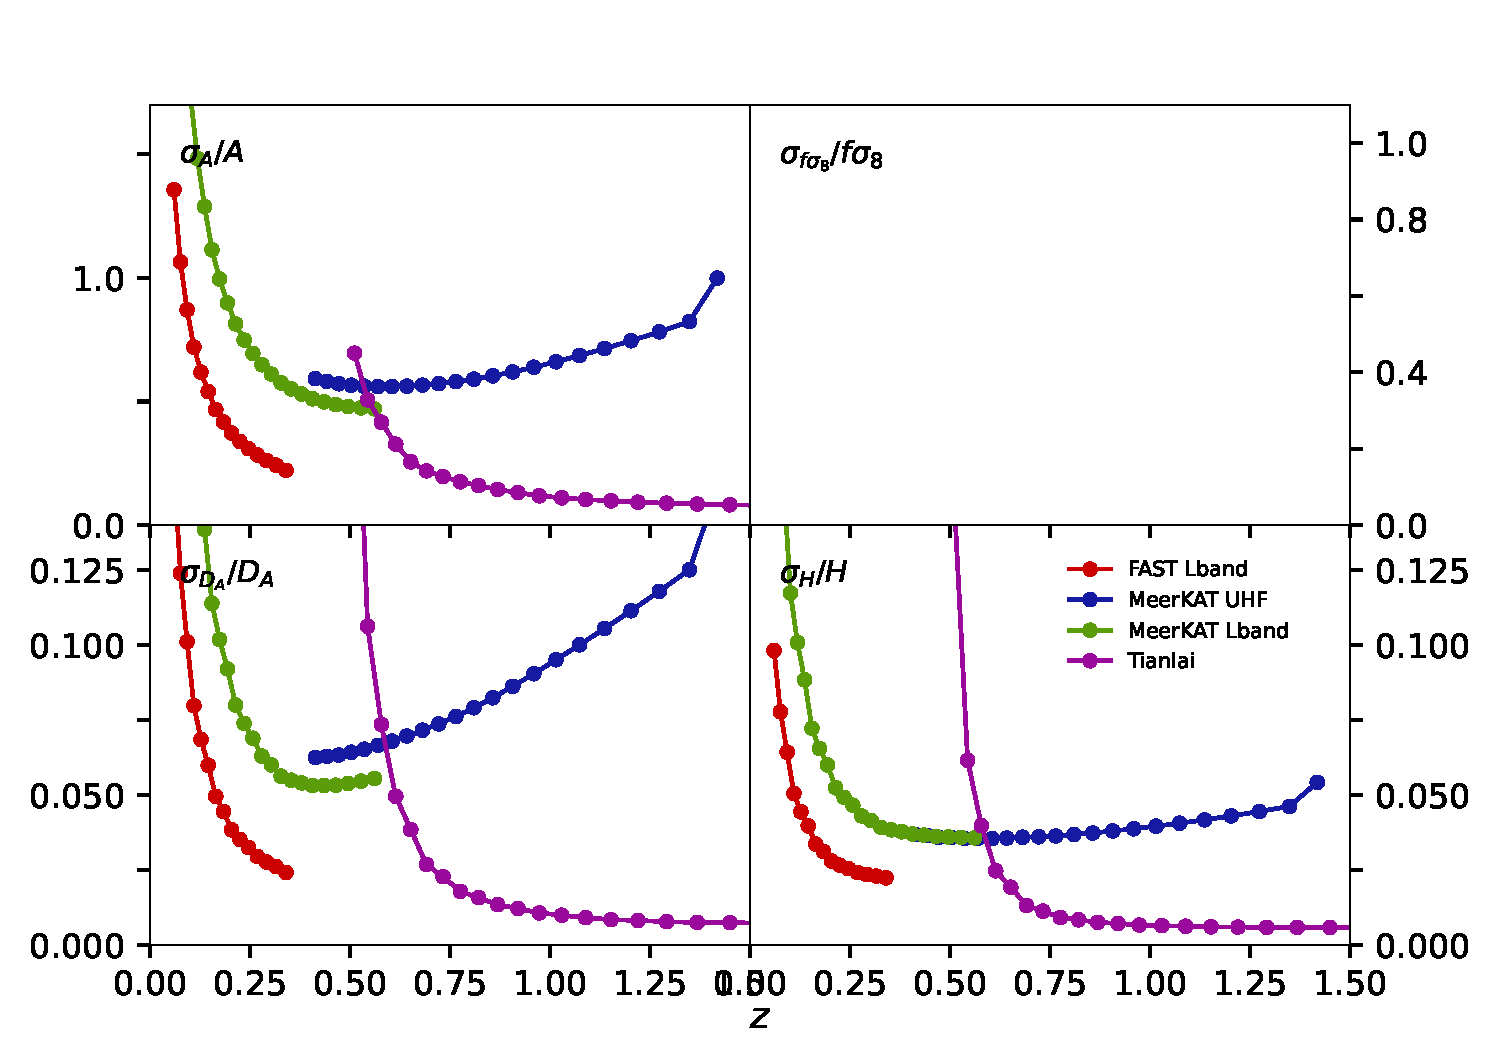
\includegraphics[scale=0.4]{fig06-zfns-FMT.pdf}
            \caption{Fractional errors on $A(z)$, $f\sigma_8(z)$(with a bug), $D_A(z)$, and $H(z)$, as a function of redshift}
        \end{figure}
    \end{frame}

    \begin{frame}
        \frametitle{}
        \begin{figure}
            \centering
            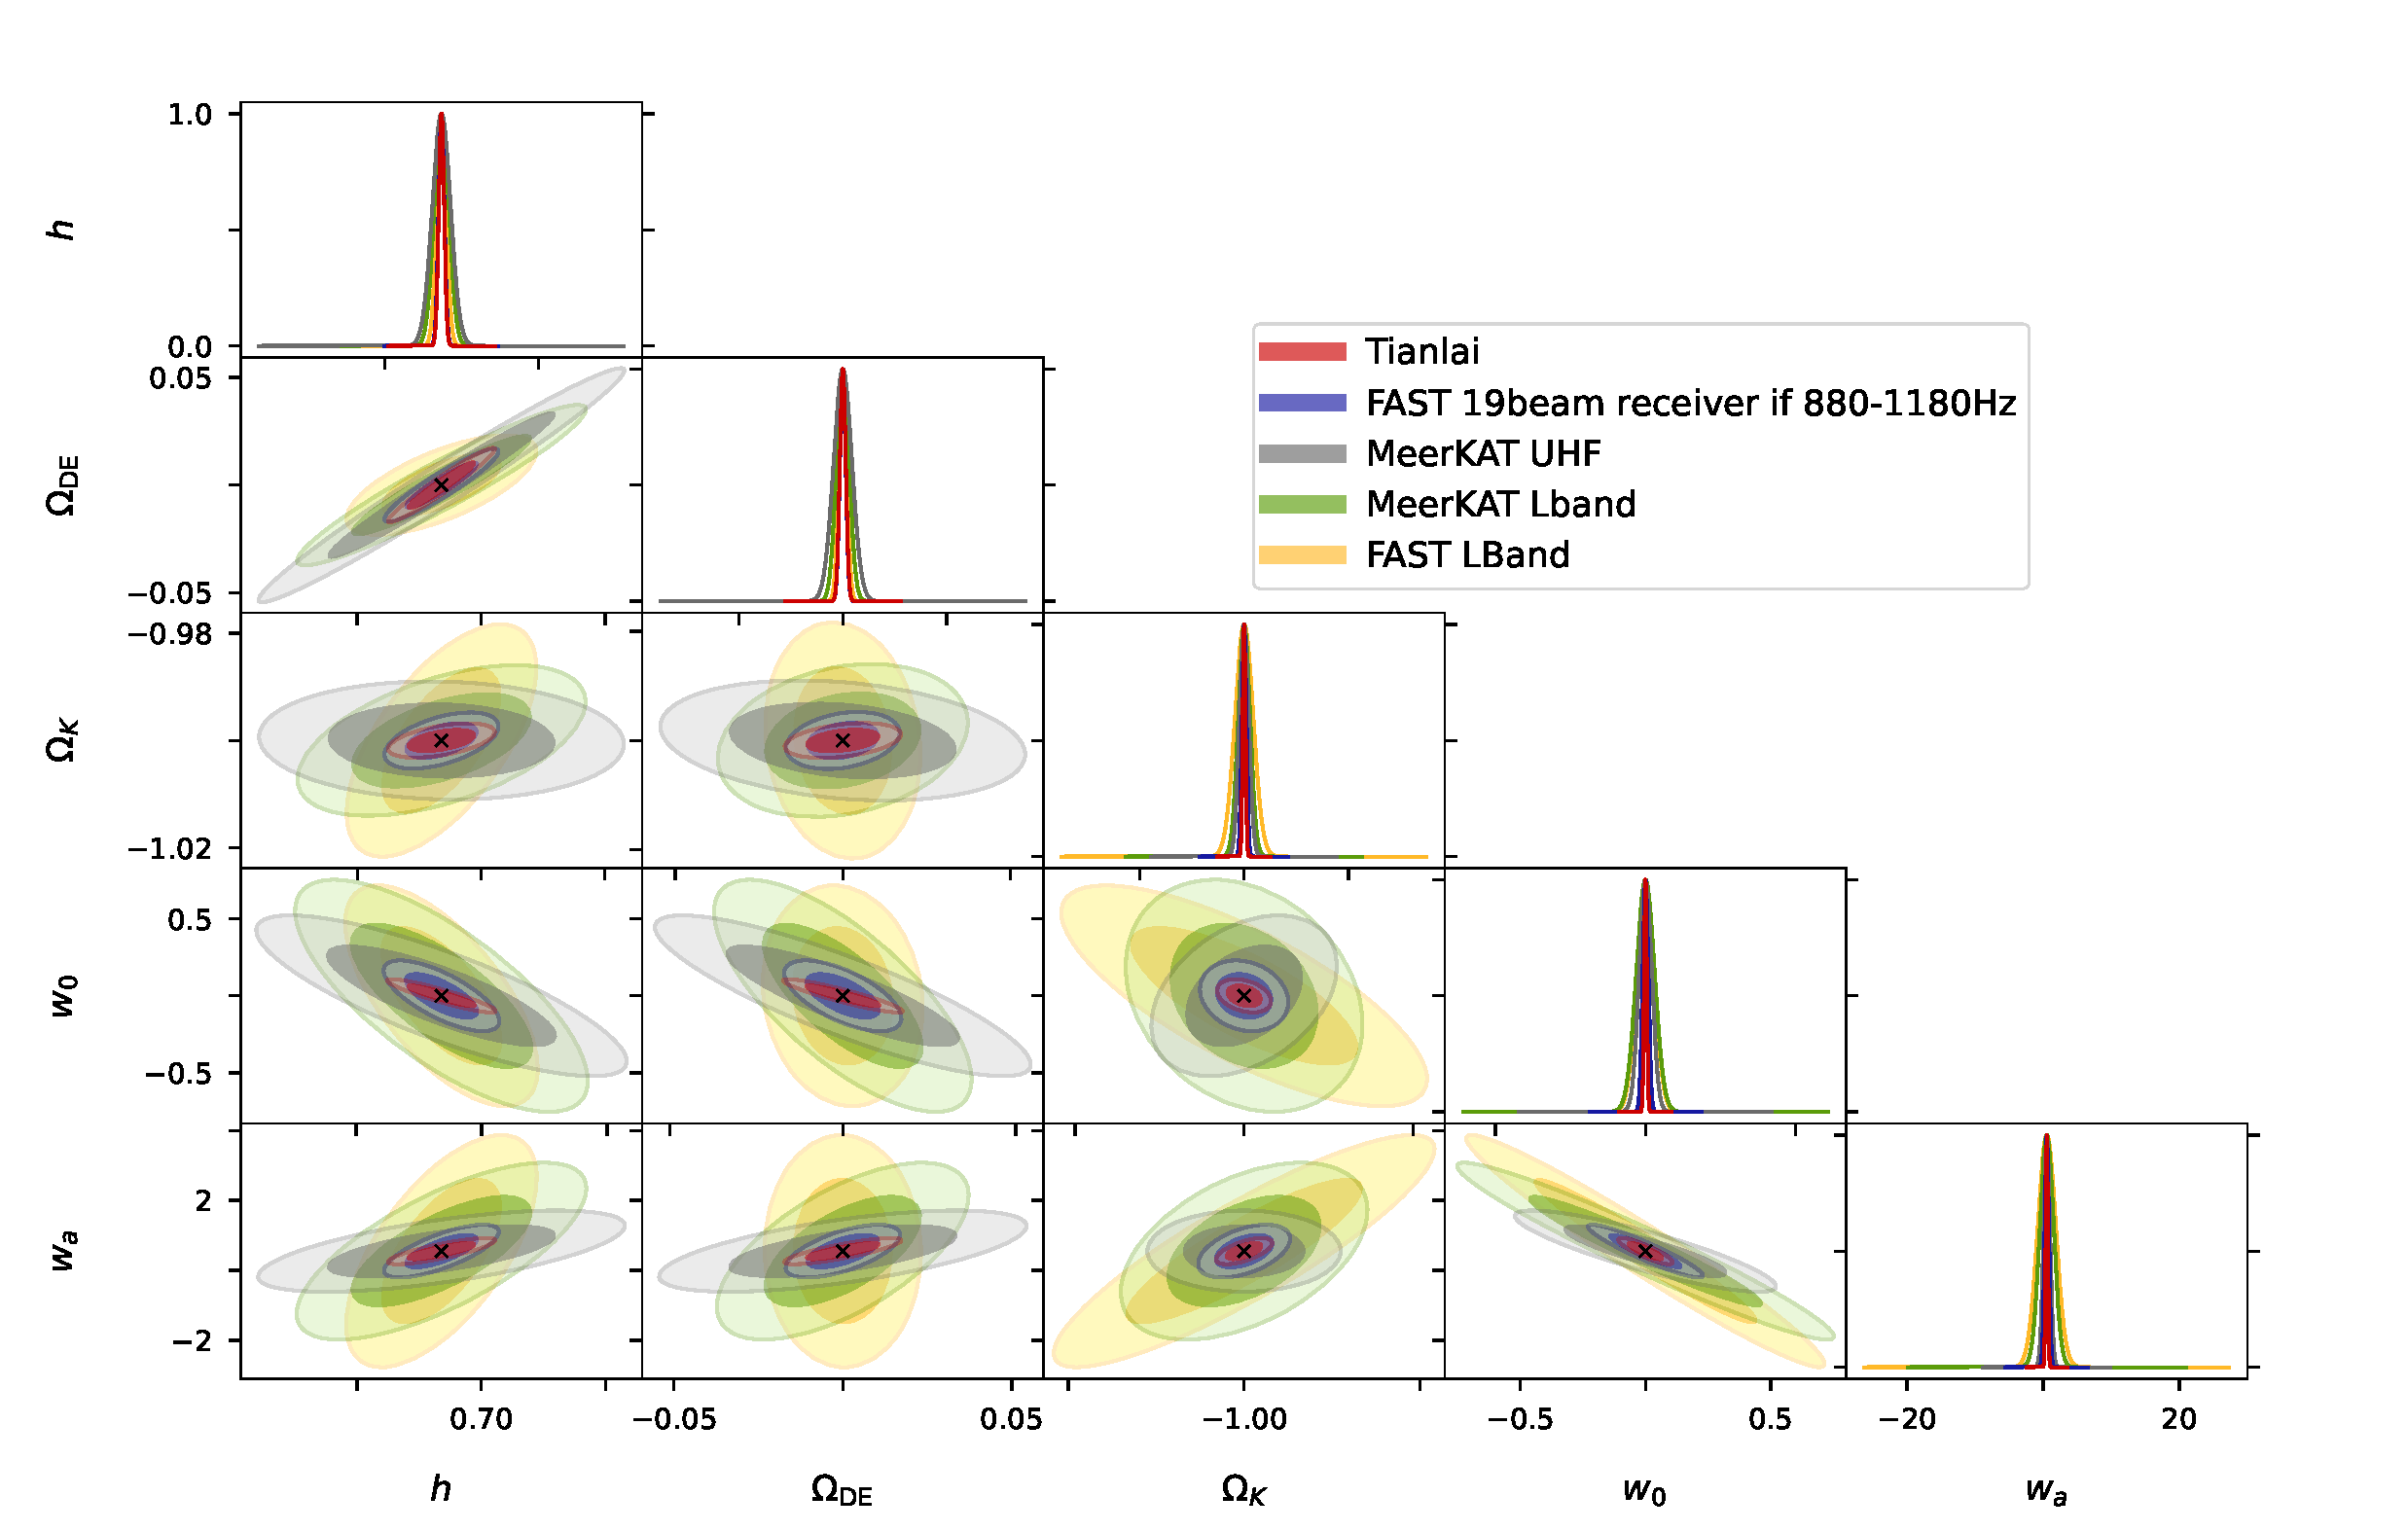
\includegraphics[scale=0.27]{fig17-6params-eos-withTianlai.pdf}
            \caption{Forecasts for dark energy and modified growth parameters (without $\gamma$)}
        \end{figure}
    \end{frame}
    \begin{frame}
        \frametitle{}
        \begin{figure}
            \centering
            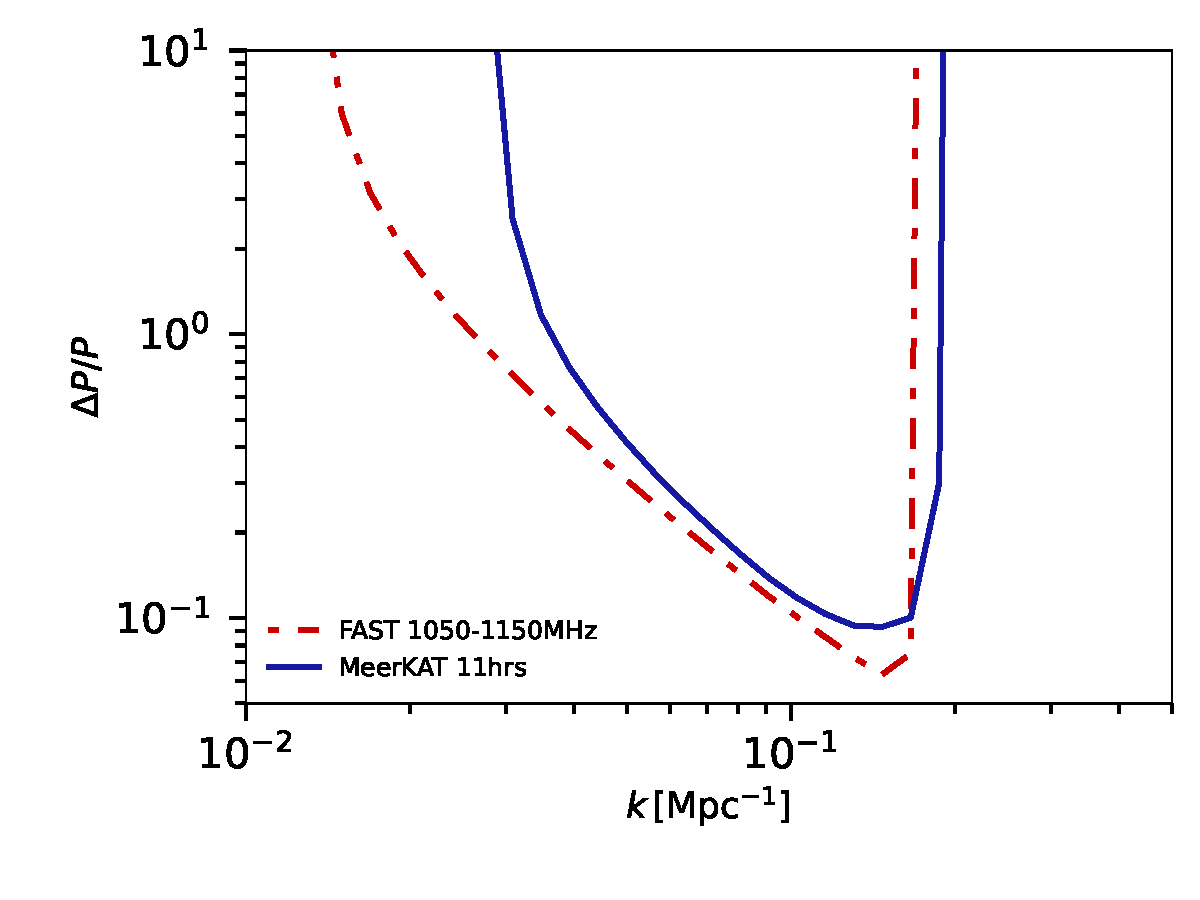
\includegraphics[scale=0.4]{fig04-dlogp-FAST-Meerkat.pdf}
            \caption{Fractional constraints on P(k) of FAST and MeerKAT 11hrs wiggleZ field}
        \end{figure}
    \end{frame}
    \begin{frame}
        \frametitle{MeerKAT 11hrs \& FAST $200deg^2$ 1050-1150MHz}
        \begin{figure}
            \centering
            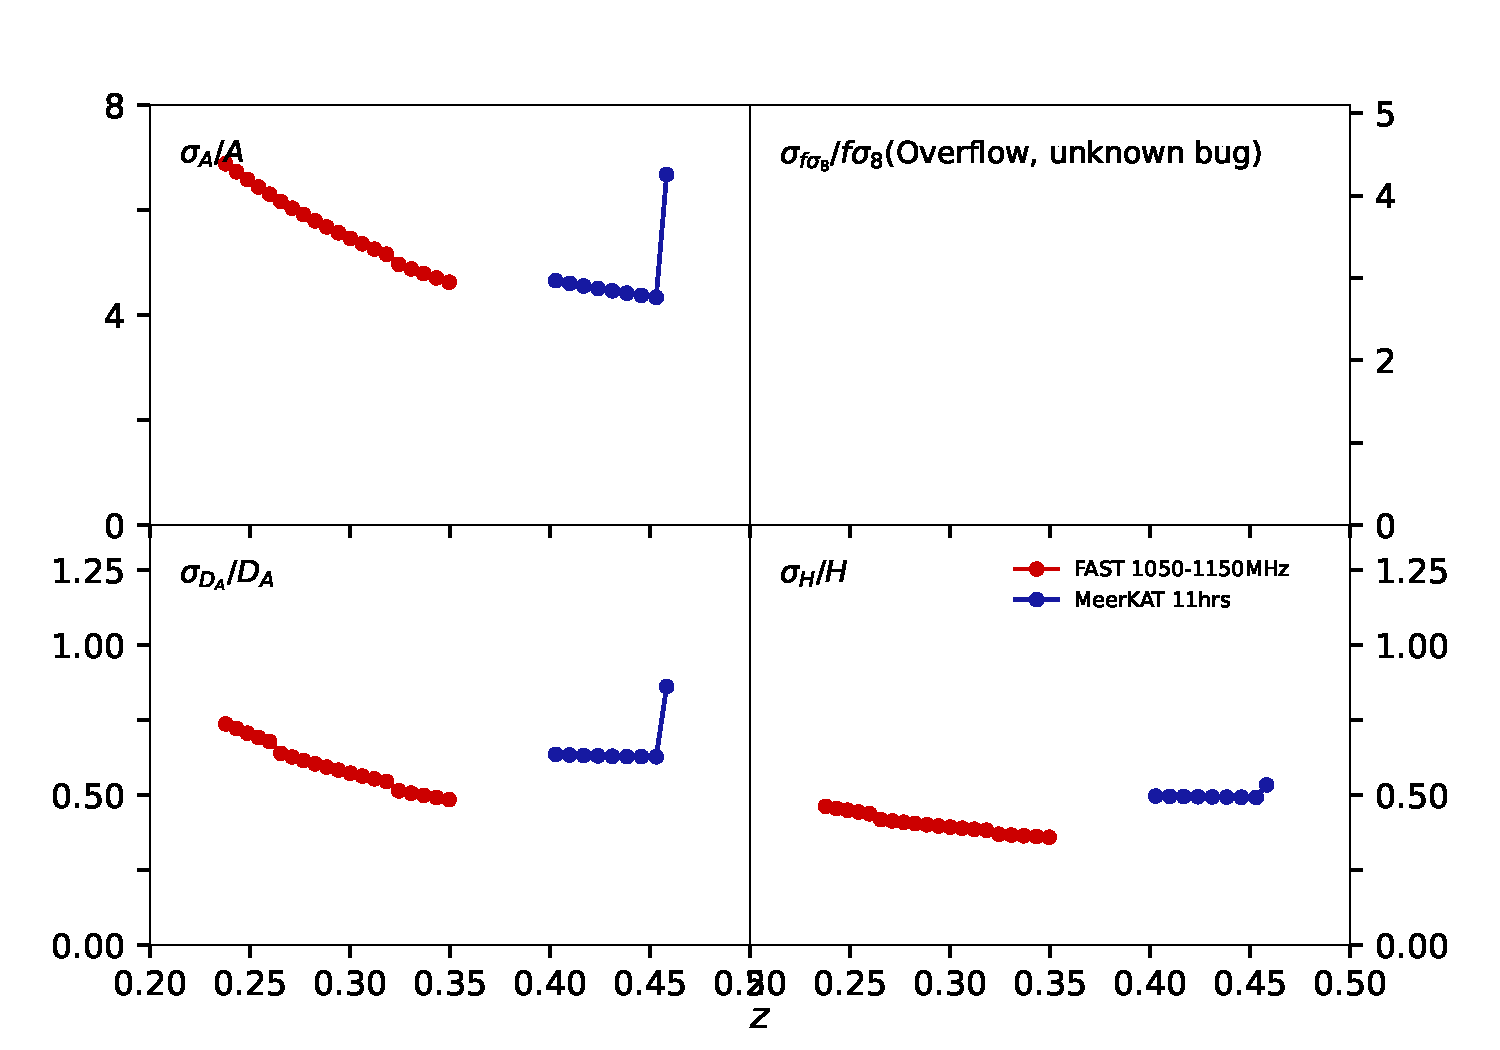
\includegraphics[scale=0.35]{fig06-zfns_FM_pre_expt.pdf}
            \caption{Fractional errors on $A(z)$, $D_A(z)$, and $H(z)$, as a function of redshift. Assuming a FAST survey with $S_{area}=200deg$ and $48/(1+z)s/pix$(DF mode scans twice)}
        \end{figure}
    \end{frame}
    

\end{document} 